\appendix
\section{Limitations}
\label{sec:limitation}
Due to the fixed-length generation requirement of LLaDA, our \grpo training is conducted with a predefined sequence length, which may constrain the model from discovering optimal reasoning paths—either concise solutions or extended chain-of-thought traces—as observed in prior autoregressive works like DeepSeek-R1. Future work could explore applying \grpo to models like Block Diffusion that support variable-length generation and enable scalable long-context RL training.

\section{Related Work}
\label{sec:related}

\paragraph{Diffusion Language Models}
While diffusion models have achieved remarkable success in the visual domain \citep{songscore, ho2020denoising}, their application to language has been limited, partly due to text's discrete nature. Initial approaches attempted to learn continuous diffusion models over textual latents \citep{austin2021structured, gulrajani2023likelihood}, but faced challenges with scalability and discretization. Masked diffusion has been established as a specific instance of discrete diffusion \citep{austin2021structured, sahoo2024simple, shi2024simplified, ou2024your,nie2024scaling}, with recent efforts scaling these models significantly. DiffuLLaMA \citep{gong2025scaling} extended this approach by initializing masked diffusion language models with pretrained LLaMA weights. \citet{yediffusion} explored how diffusion language models can generate chain-of-thought reasoning, and complex reasoning tasks on smaller-scale models~\citep{ye2024beyond}, highlighting their advantages over autoregressive models in reversal tasks, though their traces lacked self-correction capabilities. \citet{arriola2025block} proposed Block Diffusion, a hybrid approach that models sequences block-by-block while applying diffusion within each block, allowing flexible length generation and improving inference efficiency with kv-caching. Recently, LLaDA \citep{nie2025largelanguagediffusionmodels} and Dream \citep{dream2025} demonstrated that large diffusion language models can achieve performance comparable to similarly-sized autoregressive alternatives, but have not yet been enhanced through reinforcement learning. To the best of our knowledge, we are the first to demonstrate the efficacy of policy gradient-based reinforcement learning algorithms on large diffusion language models. 

\paragraph{Improving Reasoning Abilities of LLMs through SFT and RL}
Approaches to enhance reasoning capabilities in large language models generally fall into two categories: supervised finetuning and reinforcement learning. SFT on high-quality reasoning traces~\citep{yu2023metamath, numina_math_datasets, pasteropenwebmath} has shown promising results, while fewer but carefully curated reasoning datasets~\citep{ye2025limoreasoning, muennighoff2025s1, zhou2023lima} can outperform larger datasets. \citet{chu2025sft} demonstrate that SFT-based reasoning often relies on memorization rather than generalization, while RL methods achieve better transfer to novel scenarios, particularly when intermediate reasoning steps are difficult to supervise. Recently, algorithms like GRPO~\citep{guo2025deepseek, shao2024deepseekmath} enable efficient training by estimating advantages from group scores without requiring additional critic models as in PPO. \citet{guo2025deepseek} demonstrate that strong reasoning capabilities can emerge through RL even without SFT (DeepSeek-R1-Zero), producing long reasoning traces with self-reflection and verification steps that significantly improve performance on mathematical tasks. The development of strong reasoning models like R1 has in turn sparked renewed interest in SFT for smaller models using distilled reasoning traces from these expert reasoners. Datasets like OpenThoughts~\citep{openthoughts} and OpenR1-Math\footnote{\url{https://huggingface.co/datasets/open-r1/OpenR1-Math-220k}}, which contain reasoning traces from DeepSeek R1, enable smaller models to learn step-by-step problem-solving from expert demonstrations. For RL in discrete diffusion models, prior work by \citet{zekri2025fine} proposed a policy gradient framework using concrete score matching, but it relies on gradient-flow computations and does not target masked objectives. In contrast, our method is tailored to masked dLLMs with efficient policy gradient calculation and improved learning efficiency through random masking. Our work is among the first to explore improving reasoning in diffusion-based LLMs via both SFT and RL.




\newpage
\section{Masked dLLM Formulation}
\label{appendix:dllm-training}
Masked diffusion language model sequence of tokens $x_t, t \in [0,1)$, which follow a forward diffusion process $q$. This process takes as input the complete sequence $x_0$ at $t = 0$ and gradually corrupts it by randomly replacing tokens with a mask token \mask. Therefore, $x_t$ represents the sequence with increasing masking ratios in expectation. Each token in the sequence $x_t^i$ thus follows the conditional distribution,
\begin{equation}
\label{eq:forward}
    q_{t|0}(x_t | x_0) = \prod_{i = 0}^{L} q_{t|0}(x_t^i|x_0^i),
    \hspace{1cm} q_{t|0}(x_t^i|x_0^i) = \begin{cases}
                    1 - \alpha_t, & x_t^i = \mask \\
                    \alpha_t, & x_t^i = x_0^i
                 \end{cases}
\end{equation}
where $\alpha_t$ (a.k.a noise schedule) is strictly decreasing in $t$.
Simply put, at any timestep, the probability that a token transitions to the masked state is $\alpha_t$.  At the end of the forward process, i.e. at $t = 1$, all tokens are guaranteed to be masked. 

This masked sequence serves as the input for the reverse process. A key property of the forward process is that once a token transitions to the masked state, it cannot transition to any other state. Therefore, the conditional distribution from an arbitrary time step $t$ to $s$ (i.e., the reverse process), such that $0 \leq s < t \leq 1$ is given by,
\begin{equation}
    q_{s|t}(x^i_s|x_t) = \begin{cases}
                    1, & x_t^i \neq \mask,\ x_s^i = x_t^i \\
                    \frac{1 - \alpha_s}{1 - \alpha_t}, & x_t^i = \mask,\ x_s^i = \mask \\
                    \frac{\alpha_s - \alpha_t}{1 - \alpha_t}q_{0|t}(x_s^i|x_t), & x_t^i = \mask,\ x_s^i \neq \mask \\
                    0, & \text{otherwise} \\
                 \end{cases}
\end{equation}
The function $q_{0|t}(x_s^i|x_t)$ is estimated by the language model, that predicts the original token in sequence $x_0$, if it is masked in $x_t$. Notably, previous works find that the model does not require the timestep as an input \cite{} since the number of mask tokens implicitly provide this information to the model.

The model, parameterized as $f_\theta(\cdot|x_t)$ learns to predict all the masked tokens in the sequence $x_t$ simultaneously, similar to the masked language modeling task. More specifically, it is trained by minimizing a NELBO of the negative log-likelihood, given by,
\begin{equation}
    \label{eq:nelbo_general}
    \text{NELBO}(\theta) \triangleq \mathbb{E}_{x_0, x_t} \left[ \int_{t=0}^{t=1} \frac{\alpha'_t }{1 - \alpha_t} \sum_{i=1}^{L} \indicator[x_t^i = \mask] \log f_{\theta}(x_0^i \mid x_t) \right],
\end{equation}
where $x_0$ is sampled from the training data distribution $p_\text{data}$, and $x_t \sim q_{t|0}(\cdot | x_0)$. In summary, the model is trained to reverse the forward process by gradually denoising (unmasking) the input sequence (all masked tokens) and recover the data distribution.

While various forms of noise schedules can be used \citep{sahoo2024simple,shi2024simplified}, \citet[LLaDA]{nie2025largelanguagediffusionmodels} uses the linear schedule: $\alpha_t = 1 - t$. The resulting loss function is a specific form of \cref{eq:nelbo_general}:
\begin{equation}
    -\mathbb{E}_{t \sim \mathcal{U}[0,1], \, x_0, \, x_t} \left[  \frac{1}{t} \sum_{i=1}^{L} \indicator[x_t^i = \mask] \log f_{\theta}(x_0^i \mid x_t) \right].
\end{equation}






\newpage
\section{Experiment Details}
\label{appendix:training_details}

\paragraph{Inference} To decode a sequence of $N$ tokens, we use $\frac{N}{2}$ denoising steps and unmask $2$ tokens in each step.
While the decoding process can generate tokens in any order, we find that decoding from left to right in blocks yields slightly better performance in practice. This is referred to as the semi-autoregressive decoding strategy~\citep{nie2025largelanguagediffusionmodels}.
More specifically, we divide the sequence into blocks of 32 tokens. In each step, we unmask $2$ tokens with the highest confidence within the current block, regardless of their position. Once all the tokens in the current block are unmasked, we move to the next one.



\subsection{\grpo}
\label{appendix:grpo-details}

We use the TRL library~\citep{vonwerra2022trl} to implement \grpo. For our \grpo{} training, we employed Low-Rank Adaptation (LoRA) with a rank of $r=128$ and scaling factor $\alpha=64$. 

For \grpo on gsm8k, math, countdown and sudoku tasks, training was conducted on 
8 NVIDIA A100-80G GPUs, with the following hyperparameters: sequence length of 256 tokens, batch size of 6 per GPU, and gradient accumulation steps of 2. 
We optimized the model using the AdamW optimizer~\citep{loshchilov2017decoupled}, with parameters $\beta_1=0.9$, $\beta_2=0.99$, weight decay of 0.1, learning rate of $3 \times 10^{-6}$, and gradient clipping at 0.2. For computational efficiency, we utilized Flash Attention 2~\citep{dao2023flashattention2} and 4-bit quantization. In gradient update iterations, each token in the prompt is randomly masked with a probability $p_{\text{mask}} = 0.15$ for log-probability estimation. Our codebase contains further configuration details: \url{https://github.com/dllm-reasoning/d1}. We train 7700, 6600 steps (number of gradient updates) for GSM8K and MATH500 respectively; for Countdown and Sudoku, we train on synthetic generated datasets for 5000, 3800 steps respectively. 

For \grpo on coding task, training was conducted on 4 NVIDIA RTX A5000 for 7500 steps (base model + \grpo) and 9000 steps(SFT model + \grpo), with a per-device batch size of 2 and 4 gradient accumulation steps. The other hyperparameters remain the same as other tasks. Exact configuration details have been provided in our codebase.

\subsubsection{Reward Functions, RL Training, and Evaluation Datasets}

\begin{figure}[h]
    \centering
    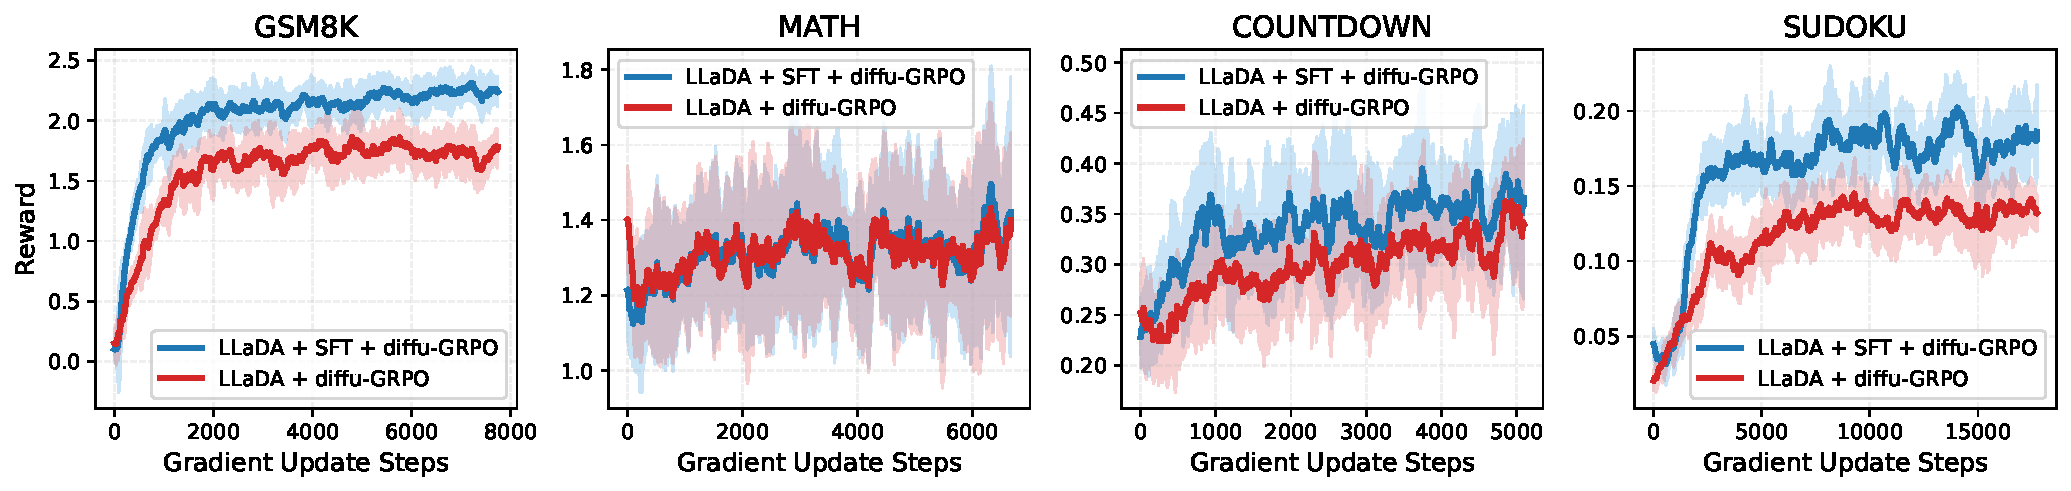
\includegraphics[width=\linewidth]{figs/rl_curves_horizontal_layout.pdf}
    \caption{Reward curves during RL training for the models in \cref{tab:performance_results}, across four reasoning tasks. We compare LLaDA+\grpo{} and \emph{d1}-LLaDA (+SFT + \grpo). \emph{d1}-LLaDA consistently achieves higher or comparable reward trajectories.}

    \label{fig:train_curves}
\end{figure}

We designed specific reward functions to guide the model's learning for each task. The rewards are structured to encourage proper formatting, accurate reasoning, and correct solutions, with varying levels of granularity depending on task requirements. We show the training curves of the results in \cref{tab:performance_results} in \cref{fig:train_curves}.

\paragraph{GSM8K}

For the GSM8K dataset, we conduct RL on the training split of the GSM8K dataset \footnote{\url{https://huggingface.co/datasets/openai/gsm8k}}and evaluate on the test split. We employ a composite reward function consisting of five components following the unsloth implementation of reward functions\footnote{\url{https://unsloth.ai/blog/r1-reasoning}}, we used these:

\begin{itemize}
    \item \textbf{XML Structure Reward}: Rewards proper formatting with reasoning and answer tags:
    \begin{itemize}
        \item +0.125 for each correctly placed opening and closing tag
        \item Small penalties for extraneous content after closing tags
    \end{itemize}
    
    \item \textbf{Soft Format Reward}: Awards 0.5 points for responses matching the pattern:
    \begin{verbatim}<reasoning>...(content)...</reasoning><answer>...(content)...</answer>\end{verbatim}
    
    \item \textbf{Strict Format Reward}: Awards 0.5 points for adhering to the exact prescribed format with appropriate line breaks.
    
    \item \textbf{Integer Answer Reward}: Awards 0.5 points if the extracted answer is a valid integer.
    
    \item \textbf{Correctness Reward}: Awards 2.0 points if the extracted answer exactly matches the ground truth.
\end{itemize}


\paragraph{Countdown}

For the Countdown task, we train on the training split of the
dataset\footnote{\url{https://huggingface.co/datasets/Jiayi-Pan/Countdown-Tasks-3to4}} 
from the TinyZero project~\citep{tinyzero}, restricting to
instances that use only three numbers. And we evaluate on 256 synthetically generated countdown questions with 3 numbers. We implement a reward function that checks if an arithmetic expression constructed from given numbers reaches a target value:

The function awards:
\begin{itemize}
    \item 1.0 point when the equation equals the target and uses exactly the available numbers
    \item 0.1 points when the equation uses the right numbers but doesn't reach the target
    \item 0 points otherwise
\end{itemize}
\paragraph{Sudoku}
% \qq{missing training dataset?}
For the 4×4 Sudoku task, we utilize the training dataset available at \url{https://github.com/Black-Phoenix/4x4-Sudoku-Dataset}, specifically the subset containing one million unique puzzles. This dataset was synthetically generated using code from \citet{arel_sudoku}. For evaluation purposes, we randomly generate 256 Sudoku puzzles using this generator.
The reward is calculated as the proportion of correctly filled cells among those that were empty in the original puzzle. This approach focuses evaluation on the model's problem-solving ability rather than its capacity to copy pre-filled values.

\paragraph{MATH500} For the MATH500 task, we train on the train split of the MATH dataset\footnote{\url{https://huggingface.co/datasets/ankner/math-500}}. Like GSM8k, we employ a composite reward function consisting of:
\begin{itemize}
    \item \textbf{Format Reward}: We award format reward points depending on the presence of  $<$answer$></$answer$>$ tags and \verb|\boxed|, as follows:
    \begin{itemize}
        \item  1.00 point if answer tags are present with \verb|\boxed| inside them
        \item 0.75 points if answer tags are present without \verb|\boxed| in them
        \item 0.50 points if answer tags are not present, but \verb|\boxed| is present
        \item 0.25 points if neither answer tags, nor \verb|\boxed| is present
    \end{itemize}
    \item \textbf{Correctness Reward}: 2.0 points if the correct answer is in \verb|\boxed{}|

\end{itemize}

\paragraph{Coding}
For the coding model, we train on the KodCode-Light-RL-10k\footnote{\url{https://huggingface.co/datasets/KodCode/KodCode-Light-RL-10K}} dataset. Again, we use a composite reward function comprising of:
\begin{itemize}
    \item \textbf{XML Structure Reward:} The same function used for GSM8k is also used for this task, with the addition that an extra 0.5 points are provided if the program is within answer tags. Additionally, 0 points are awarded if the code is not wrapped in \verb|```python```|.
    \item \textbf{Correctness Score:} Similar to \citep{gehring2024rlef, ma2025dynamic}, we use unit tests to verify the correctness of the code. Notably, while these works use a binary reward, we use the fraction of unit tests passed as the reward.
    \item \textbf{Safe Code:} To prevent the generation of unsafe code, we assign a reward of 0 if any blocked modules are used. These include \texttt{os}, \texttt{sys}, \texttt{shutil}, \texttt{subprocess}, \texttt{socket}, \texttt{psutil}, \texttt{ctypes}, \texttt{pathlib}, \texttt{builtins}, and \texttt{\_\_import\_\_}.
\end{itemize}








\subsection{SFT Details}
\label{appendix:sft-design}

\begin{algorithm}[H]
\caption{\textbf{Supervised Finetuning of LLaDA \citep{nie2025largelanguagediffusionmodels}}}
\label{alg:llada_sft}
\textbf{Require:} underlying unmasking predictor $f_{\theta}$, data distribution $p_{\text{data}}$, learning rate $\eta$ \\
\vspace{-1em}
\begin{algorithmic}[1]
\Repeat
    \State Sample $(p_0, r_0) \sim p_{\text{data}}, \quad t \sim \mathcal{U}(0,1)$ \Comment{$p_0$ is the prompt and $r_0$ is the response}
    \State Construct a partially masked response $r_t \sim q_{t|0}(r_t | r_0)$ \Comment{$q_{t|0}$ is defined in Eq. (\ref{eq:forward})}
    \State Calculate $\mathcal{L}(\theta) = -\frac{1}{t |r_0|} \sum_{i=1}^{|r_0|} \indicator[r_t^i = \mask] \log f_{\theta}(r_0^i | p_0 \oplus r_t)$
    \Comment{$\oplus$ is concatenation}
    % \hfill \# $L'$ is the sequence length of $r_0$
    \State $\theta \gets \theta - \eta \nabla_{\theta} \mathcal{L}$
\Until{Converged}
\State \textbf{Return} $\theta$
\end{algorithmic}
\end{algorithm}



Similarly, the SFT model also employs LoRA, with a rank of $r = 128$ and scaling factor $\alpha = 256$. We train with a sequence length of 4096 on 2 A6000 GPUs, using gradient accumulation over 4 steps and a per-device batch size of 1, yielding an effective batch size of 8. The optimizer and learning rate schedule match those used in \grpo{}, with a learning rate of 1e-5 and gradient clipping at 1.0. The SFT model was trained on the s1k dataset for 2460 steps, leaving 1\% of the data for evaluation. A linear learning rate decay schedule was used, with no warmup. Our codebase contains further configuration details: \url{https://github.com/dllm-reasoning/d1}.




\paragraph{Truncated Sequences} LLaDA-instruct is trained to generate full sentences, i.e., given any sequence length, it will always try to generate a complete sentence. However, due to the long sequence length of s1k, we had to truncate the dataset to have a maximum sequence length of 4096. 


\paragraph{Loss on PAD tokens} As discussed in \citet{nie2025largelanguagediffusionmodels}, LLaDA needs to take a loss on the PAD tokens to be able to effectively terminate its generation. Additionally, to speed up training, we can pad the sequences in a batch to the longest sequence length in the batch. However, in GPU-constrained environments which use a small batch size, we find that padding to the longest datapoint in the batch is suboptimal since not enough PAD tokens are considered in the loss. Therefore, we choose to pad to the max length of the model.

\paragraph{Dataset Difficulty} We find that there are some dynamics between the difficulty of the dataset and the model strength. In general, a weaker model needs a combination of easier and harder datapoints to scale reasoning. If we use an overly hard dataset, the performance degrades since the model easily overfits.


\section{Qualitative Examples on GSM8k}
\label{appendix:qualitative}
We show qualitative results from all the models. Correct answers are in \textcolor{green!70!black}{green}, incorrect answers in \textcolor{red}{red} and aha-moments in \textcolor{blue}{blue}. Notably, sometimes the model can reach the right answer via the wrong reasoning - such artifacts should reduce with a stronger base model.
\subsection{LLaDA-Instruct}
\label{appendix:qualitative-basellada}
When controlling the generation sequence length of dLLMs, it influences the reasoning style. For example, we see that with seq len = 512, compared to 128, the model produces more detailed step-by-step solutions with explicit mathematical formulas and enumerated calculations.

\begin{tcolorbox}[title=\textbf{Model:} LLaDA-8B-Instruct \\ 
\textbf{Generation Sequence Length:} 128 \\ \textbf{Question:} A 76-star flag has three rows of 8 stars\, two rows of 6 stars and the rest are 5-star rows. How many rows of 5 stars are there altogether on the flag?]
$<$reasoning$>$
The flag has three stars in 8 rows, two stars in 6 rows, and the rest are 5-star rows. The total number of stars is the sum of the stars in the three8-star rows and the 6-star rows, which is 24 + 12 = 36 stars. Therefore, the remaining 76 - 36 = 40 stars are be placed in 5-star rows. Hence, the number of 5-star rows is 40/5.
$</$reasoning$>$
$<$answer$>$
\textcolor{green!70!black}{\(\boxed{8}\)}
$</$answer$>$
\end{tcolorbox}

\begin{tcolorbox}[title=\textbf{Model:} LLaDA-8B-Instruct \\ 
\textbf{Generation Sequence Length:} 512 \\ \textbf{Question:} A 76-star flag has three rows of 8 stars\, two rows of 6 stars and the rest are 5-star rows. How many rows of 5 stars are there altogether on the flag?]
$<$reasoning$>$
To determine the number of rows of 5 stars on the 76-star flag, we need to follow these steps:

1. Calculate the total number of stars in the three rows of 8 stars.
2. Calculate the total number of stars in the two rows of 6 stars.
3. Subtract the total number of stars in the first two rows from the total number of stars on the flag to find the number of stars in the 5-star rows.
4. Divide the number of stars in the 5-star rows by 5 to find the number of 5-star rows rows.

Let's go through each step in detail:

1. The total number of stars in the three rows of 8 stars is:
   \[
   3 \times 8 = 24
   \]

2. The total number of stars in the two rows of 6 stars is:
   \[
   2 \times 6 = 12
   \]

3. The total number of stars in the first two rows is:
   \[
   24 + 12 = 36
   \]

4. The total number of stars on the flag is 76. Therefore, the number of stars in the 5-star rows is:
   \[
   76 - 36 = 40
   \]

5. The number of 5-star rows is the number of stars in the 5-star rows divided by 5:
   \[
   \frac{40}{5} = 8
   \]

So, the number of rows of 5 stars on the flag is \textcolor{green!70!black}{\(\boxed{8}\)}
$</$reasoning$>$
\end{tcolorbox}
\begin{tcolorbox}[breakable,title=\textbf{Model:} LLaDA-8B-Instruct \\ \textbf{Generation Sequence Length:} 512\\ \textbf{Question:} A bakery produces 60 loaves of bread each day. Two-thirds of the loaves are sold in the morning and half of what is left is sold equally in the afternoon and evening. How many loaves of bread are sold in the afternoon?]
$<$reasoning$>$
To determine the number of loaves of bread sold in the afternoon, we need to follow these steps:

1. Calculate the number of loaves sold in the morning.
2. Determine the number of loaves remaining after the morning sale.
3. Calculate the number of loaves sold in the afternoon and evening.
4. Identify the number of loaves sold in the afternoon.

First, we calculate the number of loaaves sold in the morning. Since two-thirds of the loaves are sold in the morning, we have:
\[
\frac{2}{3} \times 60 = 40
\]
So, 40 loaves are sold in the morning.

Next, we determine the number of loaves remaining after the morning sale. The total number of loaves produced is 60, and 40 loaves are sold morning the morning, so the number of loaves remaining is:
\[
60 - 40 = 20
\]
So, 20 loaves are after the morning sale.

Then, we calculate the number of loaves sold in the afternoon and evening. Half of the remaining loaves are sold equally in the afternoon and evening, so the number of
aves sold in the afternoon and evening is:
\[
\frac{1}{2} \times 20 = 10
\]
So, 10 loaves are sold in the afternoon and evening.

Finally, we identify the number of loaves sold in the afternoon. Since 10 loaves are sold in the afternoon and evening, and they are sold equally, the number of loaves sold in the afternoon is:
\[
\frac{10}{2} = 5
\]
So, 5 loaves are sold in the afternoon.
$</$reasoning$>
<$answer$>$
\textcolor{red}{\boxed{5}}
$</$answer$>$
\end{tcolorbox}
\subsection{SFT on Reasoning Traces from S1K}
\begin{tcolorbox}[title=\textbf{Model:} LLaDA+SFT \\ \textbf{Generation Sequence Length:} 512\\ \textbf{Question:} A 76-star flag has three rows of 8 stars\, two rows of 6 stars and the rest are 5-star rows. How many rows of 5 stars are there altogether on the flag?]
$<$reasoning$>$
To determine the number of rows of 5 stars on the 76-star flag, we need to follow these steps:

1. Calculate the total number of stars in the three rows of 8 stars.
2. Calculate the total number of stars in the two rows of 6 stars.
3. Subtract the total number of stars in the first two rows from the total number of stars on the flag to find the number of stars in the remaining rows.
4. Divide the number of stars in the remaining rows by 5 to find the number of 5-star rows.

Let's go through each step in detail:

1. Calculate the number of stars in the three rows of 8 stars:
   \[
   3 \times 8 = 24
   \]
   So, there are 24 stars in the three rows of 8 stars.

2. Calculate the number of stars in the two rows of 6 stars:
   \[
   2 \times 6 = 12
   \]
   So, there are 12 stars in the two rows of 6 stars.

3. Subtract the total number of stars in the first two rows from the total number of stars on the flag:
   \[
   76 - 24 - 12 = 40
   \]
   So, there are 40 stars in the remaining rows.

4. Divide the number of stars in the remaining rows by 5 to find the number of 5-star rows:
   \[
   \frac{40}{5} = 8
   \]
   So, there are 8 rows of 5 stars.

\textcolor{blue}{However, we need to check if the number of rows is 8, as if there are 8 rows of 5 stars, the total number of stars would be}:
\[
8 \times 5 = 40
\]
This matches the number of stars in the remaining rows, which is 40. Therefore, the number of rows of 5 stars is indeed 8.

Thus, the number of rows of 5 stars is:
\[
\boxed{8}
\]
$</$reasoning$>
<$answer$>$\textcolor{green!70!black}{\boxed{8}}$</$answer$>$
\end{tcolorbox}

\begin{tcolorbox}[float, breakable, title=\textbf{Model:} LLaDA+SFT \\ \textbf{Generation Sequence Length:} 512 \\ \textbf{Question:} A bakery produces 60 loaves of bread each day. Two-thirds of the loaves are sold in the morning and half of what is left is sold equally in the afternoon and evening. How many loaves of bread are sold in the afternoon?]
$<$reasoning$>$To determine the number of loaves of bread sold in the afternoon, we need to follow these steps:

1. Calculate the number of loaves sold in the morning.
2. Determine the number of loaves remaining after the morning sales.
3. Calculate the number of loaves sold in the afternoon and evening.
4. Identify the number of loaves sold in the afternoon.

First. Calculate the number of loaves sold in the morning:
\[ \text{Loaves sold in the morning} = \frac{2}{3} \times 60 = 40 \]

Next. Determine the number of loaves remaining after the morning sales:
\[ \text{Loaves remaining after morning sales} = 60 - 40 = 20 \]

Then. Calculate the number of loaves sold in the afternoon and evening:
\[ \text{Loaves sold in the afternoon and evening} = \frac{1}{2} \times 20 = 10 \]

Since, half of the remaining loaves are sold equally in the afternoon and evening, we need to find the number of loaves sold in the afternoon..

Finally the number of loaves sold in the afternoon is:
\[ \text{Loaves sold in the afternoon} = \frac{10}{2} = 5 \]

\textcolor{blue}{However, this seems incorrect because the problem states that half of the remaining left is sold equally in the afternoon and evening, which means the should be}:
\[ \text{Loaves sold in the afternoon} = \frac{1}{2} \times 20 = 10 \]

\textcolor{blue}{But since the problem states that half of the remaining left is sold equally in the afternoon and evening, the correct calculation should be}:
\[ \text{Loaves sold in the afternoon} = \frac{1}{2} \times 20 = 10 \]

\textcolor{blue}{However, since the problem states that half of the remaining left is sold equally in the afternoon and evening, the correct calculation should be}:
\[ \text{Loaves sold in the afternoon} = \frac{1}{2} \times 20 = 10 \]

$</$reasoning$>$
$<$answer$>$
\textcolor{green!70!black}{\boxed{10}}
$</$answer$>$
\end{tcolorbox}
\clearpage
\newpage
\subsection{\grpo}
\begin{tcolorbox}[float, breakable, title=\textbf{Model:} LLaDA+\grpo \\ \textbf{Generation Sequence Length:} 512 \\ \textbf{Question:} A 76-star flag has three rows of 8 stars\, two rows of 6 stars and the rest are 5-star rows. How many rows of 5 stars are there altogether on the flag?]
$<$reasoning$>$
To determine the number of rows of 5 stars on the flag, we first need to calculate the total number of stars in the rows with 8 stars and 6 stars. 

1. There are number of rows with 8 stars: \(3 \times 8 = 24\) stars.

2. There are number of rows with 6 stars: \(2 \times 6 = 12\) stars.

3. The these rows rows together have \(24 + 12 = 36\) stars.

Next, we need the total number of stars on the flag, which is 76. We subtract the number of stars in the rows with 8 stars and 6 stars from the total number of stars:

\[ 76 - 36 = 40 \]

So, there are 40 stars in the rows with 5 stars. To find the number of rows of 5 stars, we divide the number of stars in these rows by the number of stars per row:

\[ \frac{40}{5} = 8 \]

Therefore, there are 8 rows of 5 stars on the flag.

$</$reasoning$>
<$answer$>$
\textcolor{green!70!black}{\boxed{8}}
$</$answer$>$

\end{tcolorbox}
\begin{tcolorbox}[title=\textbf{Model:} LLaDA+\grpo \\ \textbf{Generation Sequence Length:} 512 \\ \textbf{Question:} A bakery produces 60 loaves of bread each day. Two-thirds of the loaves are sold in the morning and half of what is left is sold equally in the afternoon and evening. How many loaves of bread are sold in the afternoon?]
The bakery produces 60 loaves of bread each day. Two-thirds of the loaves are sold in the morning, so we calculate \(\frac{2}{3} \times 60 = 40\) loaves sold in the morning. After the morning sales, there are \(60 - 40 = 20\) loaves left. Half of these remaining loaves are sold equally in the afternoon and evening, so we calculate \(\frac{1}{2} \times 20 = 10\) loaves sold in the afternoon. Therefore$</$reasoning$>
<$answer$>$
\textcolor{red}{\boxed{10}}
$</$answer$>$

\end{tcolorbox}
\clearpage
\newpage
\subsection{\emph{d1}-LLaDA}
\begin{tcolorbox}[breakable, float, title=\textbf{Model:} \emph{d1}-LLaDA \\ \textbf{Generation Sequence Length:} 512 \\ \textbf{Question:} A 76-star flag has three rows of 8 stars\, two rows of 6 stars and the rest are 5-star rows. How many rows of 5 stars are there altogether on the flag?]
$<$reasoning$>$
To determine the number of rows of 5 stars on a 76-star flag, we need to follow these steps:

1. Calculate the total number of stars in the three rows of 8 stars.
2. Calculate the total number of stars in the two rows of 6 stars.
3. Subtract the total number of stars in the first two rows from the total number of stars on the flag to find the number of stars in the remaining rows.
4. Divide the number of stars in the remaining rows by the number of stars per row to find the number of rows of 5 stars.

Let's go through each step in detail:

1. The total number of stars in the three rows of 8 stars is:
   \[
   3 \times 8 = 24
   \]

2. The total number of stars in the two rows of 6 stars is:
   \[
   2 \times 6 = 12
   \]

3. The total number of stars in the first two rows is:
   \[
   24 + 12 = 36
   \]

4. Subtract the total number of stars in the first two rows from the total number of stars on the flag:
   \[
   76 - 36 = 40
   \]

5. Divide the number of stars in the remaining rows by the number of stars per row to find the number of rows of 5 stars:
   \[
   \frac{40}{5} = 8
   \]

Therefore, there are 8 rows of five stars on the flag.
$</$reasoning$>
<$answer$>$
\textcolor{green!70!black}{\boxed{8}}
$</$answer$>$

\end{tcolorbox}
\begin{tcolorbox}[float,breakable,title=\textbf{Question:} Jennifer's dog has 8 puppies\, 3 of which have spots. Brandon's dog has 12 puppies\, 4 of which have spots. What percentage of all the puppies have spots?]
$<$reasoning$>$
To determine the percentage of all the puppies that have spots, we need to follow these steps:

1. Calculate the total number of puppies from both dogs.

2. Calculate the total number of puppies with spots from both dogs.

3. Determine the percentage of puppies with spots.

First, let's find the total number of puppies from both dogs:

- Jennifer's dog has 8 puppies.

- Brandon's dog has 12 puppies.

- Total number of puppies = 8 + 12 = 20.

Next, let's find the total number of puppies with spots from both dogs:

- Jennifer's dog has 3 puppies with spots.

- Brandon's dog has 4 puppies with spots.

- Total number of puppies with spots = 3 + 4 = 7.

Now, we need to determine the percentage of puppies with spots. The formula for percentage is:
\[ \text{Percentage} = \left( \frac{\text{Number of puppies with spots}}{\text{Total number of puppies}} \right) \times 100 \]

Substituting the values we have:
\[ \text{Percentage} = \left( \frac{7}{20} \right) \times 100 \]

To simplify the fraction, we find the greatest common divisor (GCD) of 7 and 20, which is 1.
\[ \frac{7}{20} = 7 \div 20\]

\textcolor{blue}{However, it seems there was a mistake in the calculation. Let's recheck the steps.}

1. Total number of puppies = 8 + 12 = 20.

2. Total number of puppies with spots = 3 + 4 = 7.

3. Percentage of puppies with spots = \(\left( \frac{7}{20} \right) \times 100\).

Let's calculate the percentage correctly:
\[ \text{Percentage} = \left( \frac{7}{20} \right) \times 100 = \frac{7 \times 100}{20} = \frac{700}{20} = 35 \]

The calculation answer.
$</$reasoning$>
<$answer$>$
\textcolor{green!70!black}{\boxed{35}}
$</$answer$>$

\end{tcolorbox}

% \begin{tcolorbox}[float, breakable, title=\textbf{Model:} \emph{d1}-LLaDA \\ \textbf{Generation Sequence Length:} 128\\ \textbf{Question:} A bakery produces 60 loaves of bread each day. Two-thirds of the loaves are sold in the morning and half of what is left is sold equally in the afternoon and evening. How many loaves of bread are sold in the afternoon?]
% $<$reasoning$>$    
% The bakery produces 60 loaves of bread each day. Two-thirds of the loaves are sold in the morning, which is $2{/}3 \times 60 = 40$ loaves. After the morning sales, there are $60 - 40 = 20$ loaves left. Half of what is loaves left is sold equally in the afternoon and evening, so $20{/}2 = 10$ loaves are sold in the afternoon.
% $</$reasoning$>$
% $<$answer$>$
% \textcolor{red}{\boxed{10}}
% $</$answer$>$
% \end{tcolorbox}

\begin{tcolorbox}[float, breakable, title=\textbf{Model:} \emph{d1}-LLaDA \\ \textbf{Generation Sequence Length:} 512\\ \textbf{Question:} A bakery produces 60 loaves of bread each day. Two-thirds of the loaves are sold in the morning and half of what is left is sold equally in the afternoon and evening. How many loaves of bread are sold in the afternoon?]
$<$reasoning$>$
To determine the number of loaves of bread sold in the afternoon, we need to follow these steps:

1. Calculate the number of loaves sold in the morning.
2. Determine the number of loaves remaining after the morning sale.
3. Calculate the number of loaves sold in the afternoon and evening.
4. Identify the number of loaves sold in the afternoon.

Let's start by calculating the number of loaves sold in the morning. The bakery sells two-thirds of the loaves in the morning.
\[
\text{Loaves sold in the morning} = \frac{2}{3} \times 60 = 40
\]
Since we can't sell a fraction of whole loaves, we assume the problem implies for the integer part of the calculation.

So, the loaves sold in the morning are 40.

Next, we determine the number of loaves remaining after the morning sale.
\[
\text{Loaves remaining after morning sale} = 60 - 40 = 20
\]

Now, we calculate the number of loaves sold in the afternoon and evening. Half of the remaining loaves are sold equally in the afternoon and evening.
\[
\text{Loaves sold in the afternoon and evening} = \frac{1}{2} \times 20 = 10
\]

\textcolor{blue}{Since the problem asks for the number of loaves sold in the afternoon, we need the integer part of the division.}
\[
\text{Loaves sold in the afternoon} = \frac{10}{2} = 5
\]

Therefore, the number of loaves of bread sold in the afternoon is \boxed{5}.
$</$reasoning$>$
$<$answer$>$
\textcolor{green!70!black}{\boxed{5}}
$</$answer$>$
\end{tcolorbox}
